%% The following is a directive for TeXShop to indicate the main file
%%!TEX root = diss.tex

\chapter{A Problem Space of 3D Reconstruction}
\label{ch:3DRecon_ProbSpace}
We discussed the current landscape of 3D reconstruction in Chapter~\ref{ch:RelatedWork}. Previous research has been solely focused on developing novel algorithms and softwares to tackle this problem. Most research efforts have been devoted to improve algorithmic performance in terms of accuracy, speed, or relax assumptions so that they can be applied to more general situations. However, this approach, which is called \textit{algorithm-center} approach, faces one big challenge: it provides little to none insight to the conditions that allow a specific algorithm to work well. This knowledge is either unknown or largely empirical, with each algorithm mapped roughly to a sub-volume in the problem space that is poorly defined, thus requires vision knowledge to fully take advantage of these algorithms. The reasons for creating this challenge are that 1) compared to developing algorithmic novelties, it is generally a neglected research direction to discover the problem conditions of existing algorithms; 2) the problem space is poor defined, there is no way of describing the problem conditions in the first place. We argue below that this is a critical part of designing an interface to 3D reconstruction, and should receive more research efforts. 

We have established in Chapter~\ref{ch:RelatedWork} that most 3D vision algorithms only targets a limited set of problem conditions, thus they are unsuitable to reconstruct objects with a wide range of properties. It might work for one condition, but is highly likely to fail on another condition. Thus, it is crucial to have multiple algorithms, each is registered to a distinct sub-volumn in problem space when it comes to design an interface to 3D reconstruction problem. To achieve this goal, first and foremost, we need a better understanding of the problem space. More specifically, we need to be able to describe the key characteristics of an object that are crucial for reconstruction. For instance, instead of describe a cup as merely a cup, we should be much more specific, and desceibe it as a white, glossy porcelain cup with shallow strips on the surface. Note we have specifically focused on the material and geometric properties of the objects, as they are the cues used by many vision algorithms, but also the key components of the problem space. It then becomes possible to evaluate the performance of algorithms under this well-defined conditions, which generates a one-to-one relation between problem space and algorithms. We call it the \textit{problem-centered} approach. This approach transforms the 3D reconstruction problem from one requiring knowledge and expertise of specific algorithms in terms of \textit{how} and \textit{where} to use them, to one requiring knowledge of problem conditions, which can be perceptually estimated or measurable.

In this chapter, we first propose a well-defined problem space consisting of reflective and geometric properties. What we mean by problem space is a accumulative space occupied by different visual and geometric properties and all their combinations. The problem space is generally too vast to tackle, thus we state addition assumptions and underlying rationales to limit the scope of the problem. Finally, we propose four main problem conditions that we are interested in investigating in this thesis.

% First, we need to have a better understanding of the problem space. In this thesis, what we mean problem space is the volume of reflectance and shape variations that objects occupy. We first describe the visual and geometric properties that constitute this problem space, then we provide further discussions regarding additional assumptions and underlying rationales to further narrow the problem space, and propose the 

% Developers started to come up with applications and working scenarios that are suitable for the developed algorithms. This approach to problem solving leads to so many examples of excellent technology, yet poor applications. The scientific approach to problem solving starts with defining the problem of interest. Without a formal understanding of the problem space, any efforts towards solving the problem have the risk of getting stuck in a deadend or diverging into a totally different and irrelevant direction and ending up with an undesired solution. The same logic applies to the research on 3D reconstruction. Thus, this chapter sets out to gives a comprehensive definition to the field of 3D reconstruction, and states additional assumptions to narrow the problem space so that it can be tackle within this thesis.

\section{Problem space}
We first give an overview of problem space, which consists of visual and geometric properties of real-world objects, as shown in Figure~\ref{fig:obj_class}. These properties can be conceptualized as dimensions/axes of the 3D reconstruction problem space. This approach allows us to think of algorithms pointing to volumes within an $n-$dimensional problem space. Existing algorithms can be incorporated into the interface by evaluating the algorithmic performance within the problem space, as shown in Figure~\ref{fig:embed_algo}. However, by no means are the presented problem space complete. There are many other properties not included that are commonely seen in the real world. For instance, properties such as metalness, emission, occlusion, discontinuity, among others, are not considered. However, the listed set of properties are broad enough to encompass a wide range of real-world objects. To help easy identification of a specific problem condition, we propose the following labels to differentiate object classes.
\begin{figure}[!htbp]
\centering
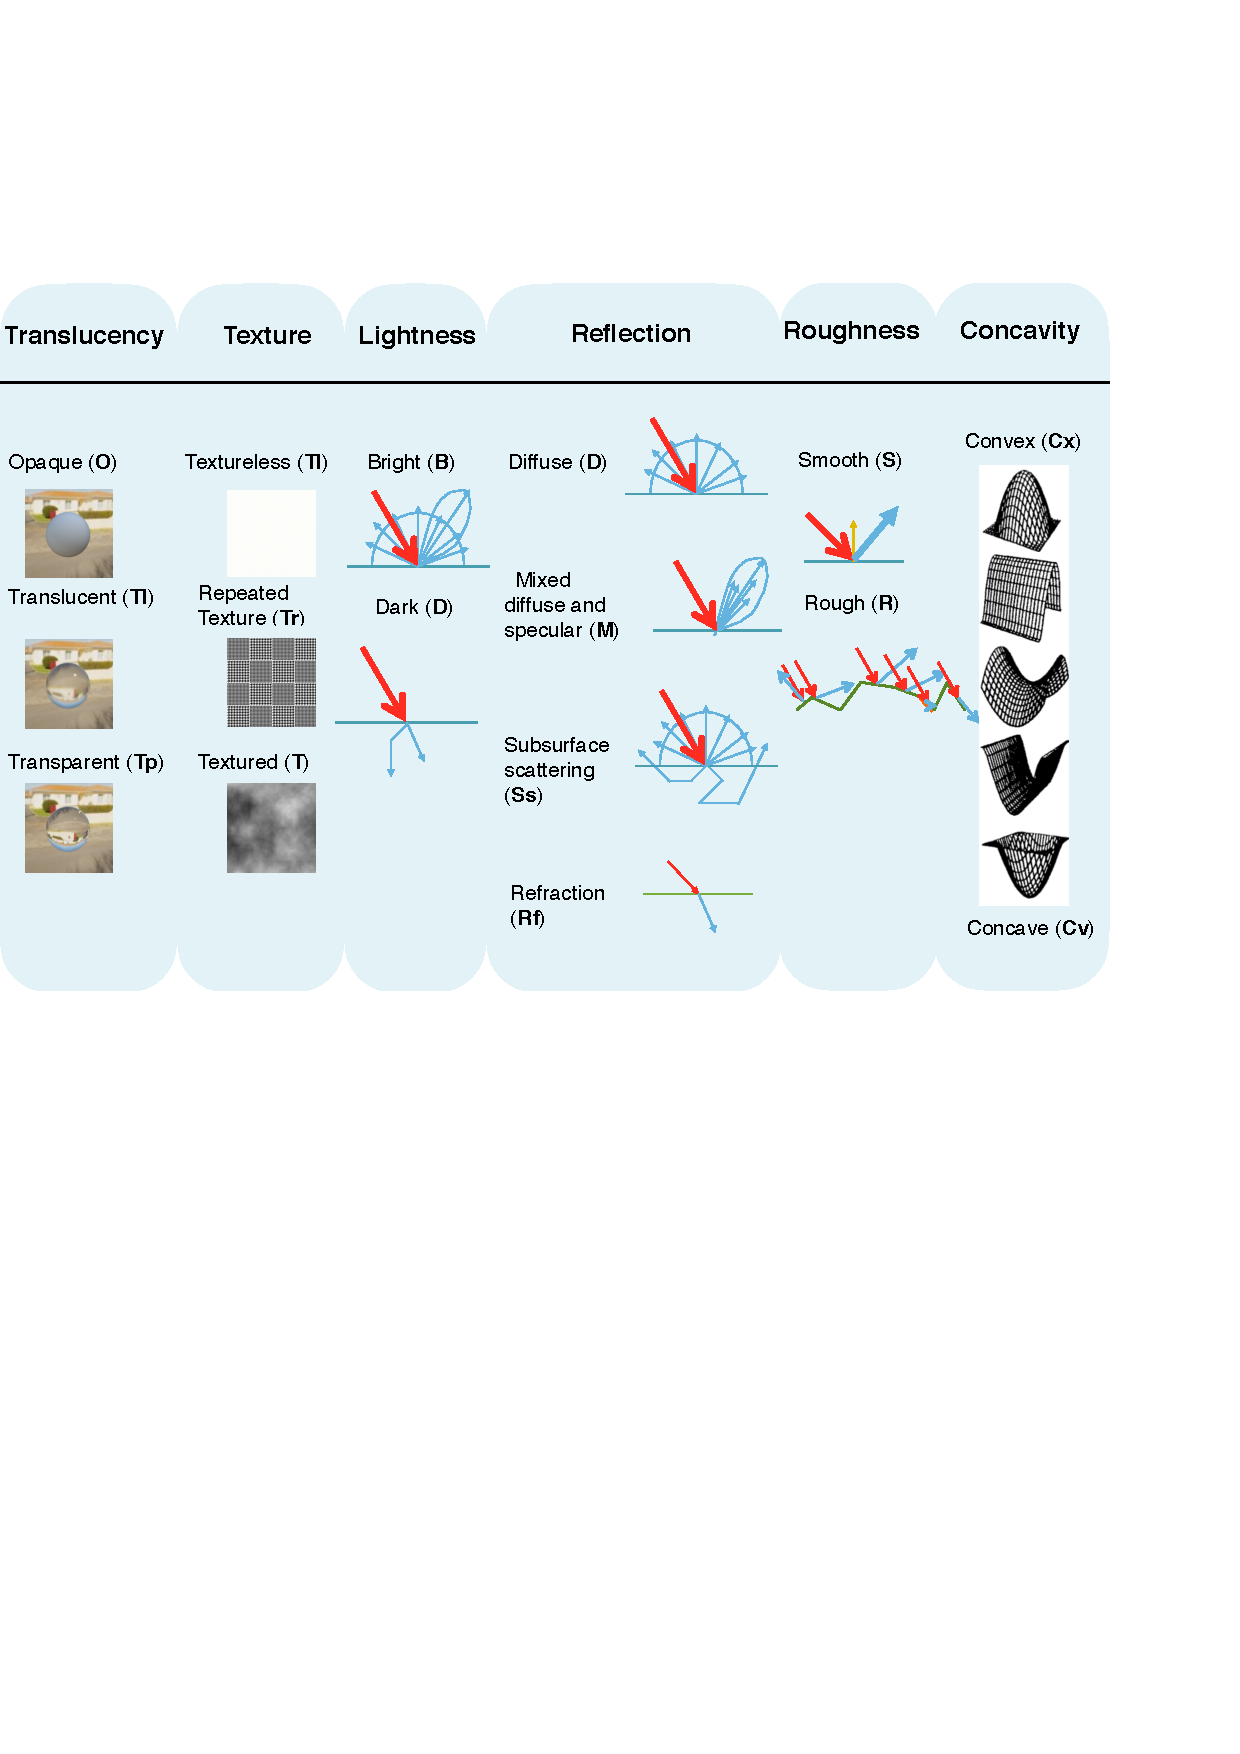
\includegraphics[width=\textwidth]{prob_space/obj_class}\\
\caption{A list of properties for object classes.}
\label{fig:obj_class}
\end{figure}

\subsubsection{Labels of Properties}
\begin{itemize}
\item \textbf{Translucency}: \textbf{O}: opaque, \textbf{Tl}: translucent, \textbf{Tp}: transparent.
\item \textbf{Texture}: \textbf{T}: textured, \textbf{Tr}: repeated textured, \textbf{Tl}: textureless.
\item \textbf{Lightness}: \textbf{B}: bright, \textbf{D}: dark.
\item \textbf{Reflection}: \textbf{D}: diffuse model, \textbf{S}: specular model, \textbf{M}: mixture of diffuse and specular, \textbf{Ss}: subsurface scattering, \textbf{Rf}: refraction
\item \textbf{Roughness}: \textbf{S}: smooth, \textbf{R}: rough
\item \textbf{Concavity}: \textbf{Cx}: convex, \textbf{Cv}: concave
\end{itemize}

\section{Assumptions}
To limit the scope of this work, we make the following assumptions:

\subsection{Simplified light interaction model}
We assume \textbf{local interaction model}, \ie global light transport such as transmission, refraction, cast shadow, inter-reflection, metalic are not considered. The rationale behind our choice is that most techniques that have been developed over the past few decades mainly tackle object with an opaque, diffuse or mixed surface. For specular, refractive, and translucent or transparent objects, only very specialized algorithms are applicable for reconstruction~\cite{ihrke2010transparent}. This is a widely used and accepted model in varied areas of computer vision, including shape from stereo, shading, and so on. As more algorithms become available to tackle these types of objects, they can be embedded to the interface using the same approach will be discussed in Chapter~\ref{ch:3DRecon_Mapping}, as shown in Figure~\ref{fig:embed_algo}.
\begin{figure*}[!htbp]
\centering
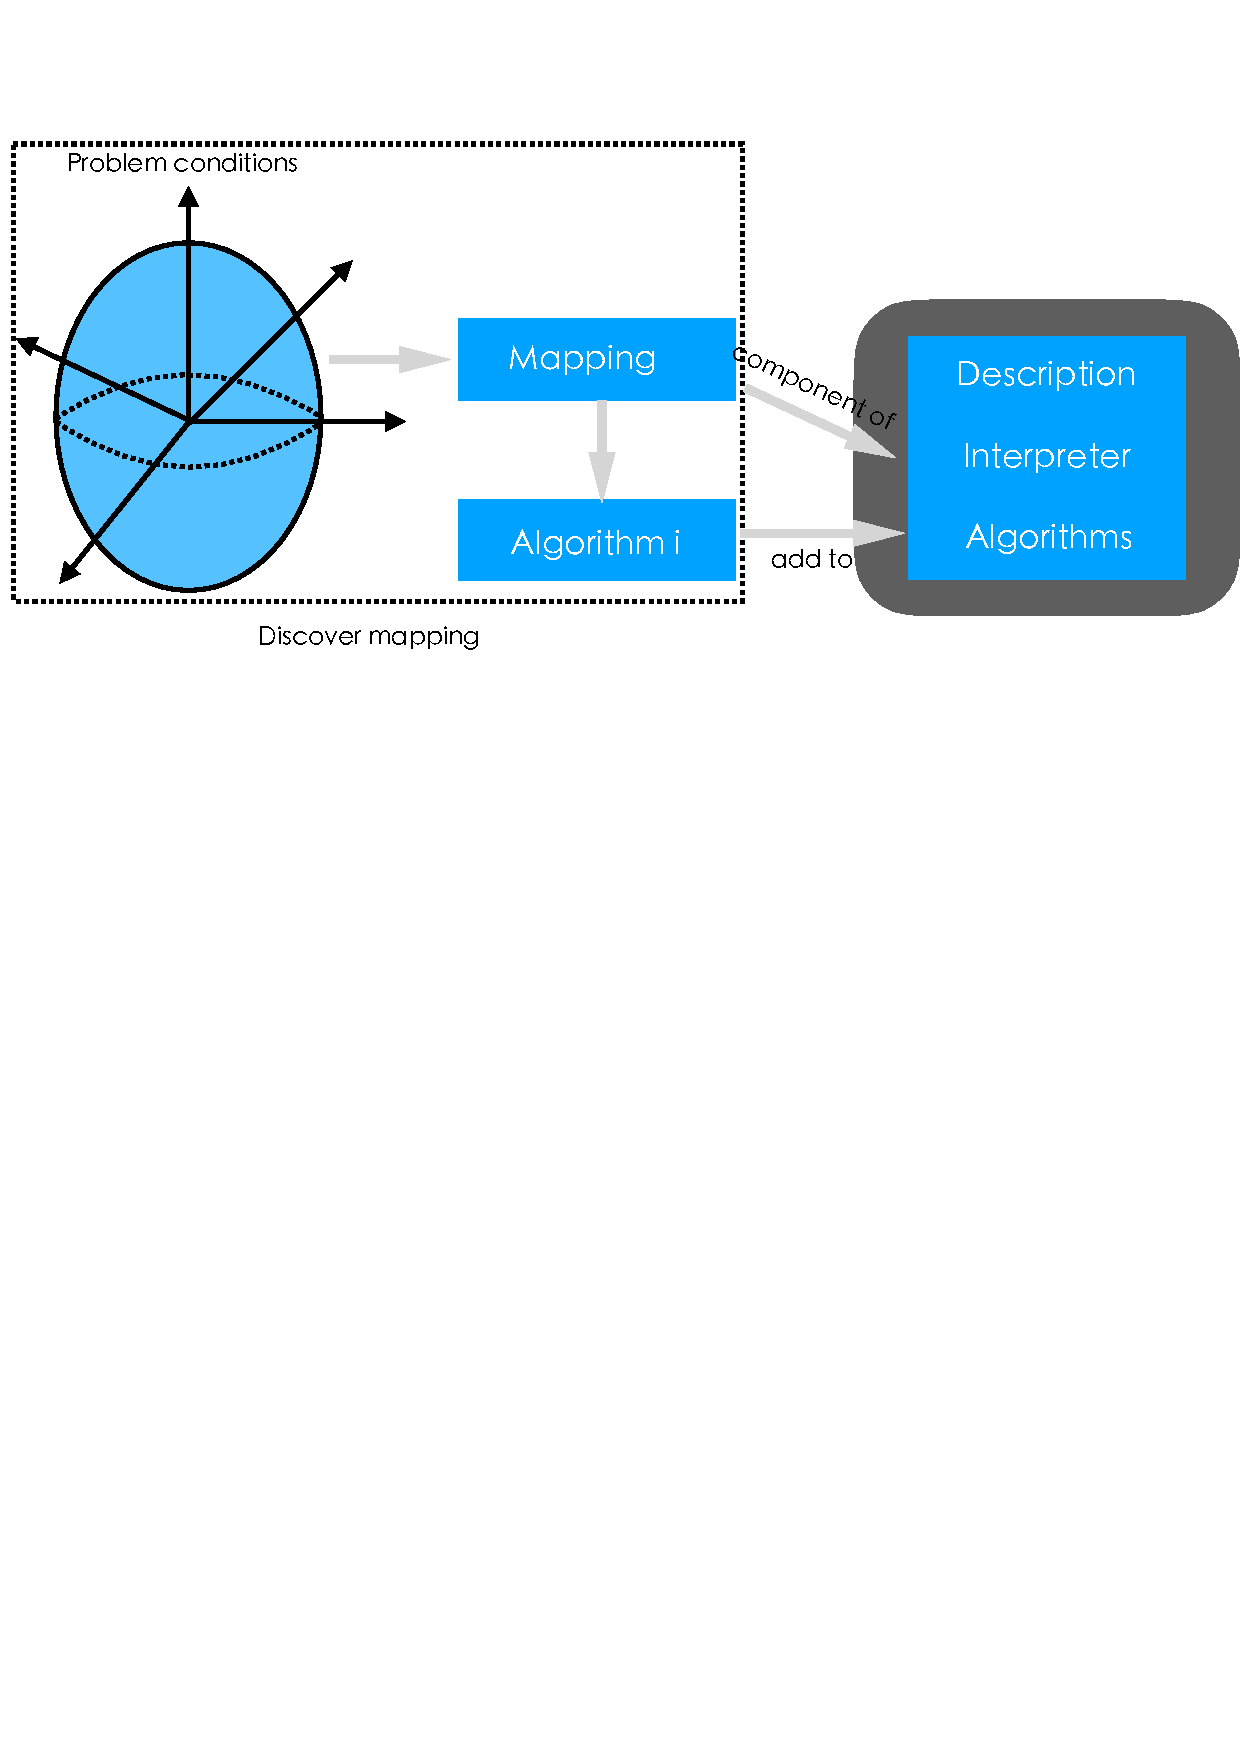
\includegraphics[width=0.8\textwidth]{img/prob_space/embed_algo.pdf}
\caption{Embed algorithms into the interface.}
\label{fig:embed_algo}
\end{figure*}

\subsection{Simplified reflectance model}
Since the majority of reconstruciton techniques rely on observing light reflected off a surface, surfaces exhibit significant effect of global light tranport present a huge challenge to the reconstruction problem. Surface exhibits global light transport, including \textit{specular}, \textit{transmission}, \textit{sub-surface scattering}, \textit{inter-reflection}, \textit{self-shadow}, and etc would break the assumptions made by most generic 3D reconstruction algorithms. Thus the global light transport are ignored, and the reflection properties of consideration are \textit{albedo}, \ie the ratio of reflected light w.r.t the received light, and \textit{specularity}, \ie the amount of specular reflection. A more comprehensive model should be constructed based on our work to incorporate more complex phenomena to be more comprehensive.

\subsection{Simplified geometric model}
It's a challenging task to model geometry using mathematical descriptions. For geometric primitives such as cube, sphere, or cone, etc, it's possible to describe the shape using concise descriptions. However, the task becomes prohibitive when it comes to shapes with varied characteristics. Furthermore it becomes more ambiguous when natural language is employed. Thus we only consider the microscopic roughness of the surface, which has a direct relation with the reflection. Other prominent geometric properties such as \textit{concavity}, which affects self-shadow, inter-reflection, \textit{depth-discontinuity}, which affects the depth estimation, are ignored.

\subsection{Simplified surface albedo}
Existing 3D vision techniques requires distinct cues for reconstruction, be it texture, intensity variation, focus change, and so on. This information will become much noisier and less effective on dark surfaces. Surfaces with low albedo will effectively eliminate some possible candidate algorithms including most active techniques. This works fine since only one algorithm is required to be returned by the interface. However, as an demonstrative purpose, it causes speculations as whether the lack of is due to the interface or the challenging nature of the dark surface. To better demonstrate the effectiveness of the interface, we decide to focus on bright surfaces. By making this assumption, we can avoid eliminate multiple algorithms in the first place, and see if the interpreter can pick the right one based on user's description.

\section{Four problem conditions}
\label{sec:four_prob_cond}
Four classes of problem conditions are being investigated in depth, as shown in Figure~\ref{fig:prob_cond}. They are selected based on the assumptions, availability of reliable techniques and the diversity of corresponding real-world objects.
\begin{figure*}[!htbp]
\centering
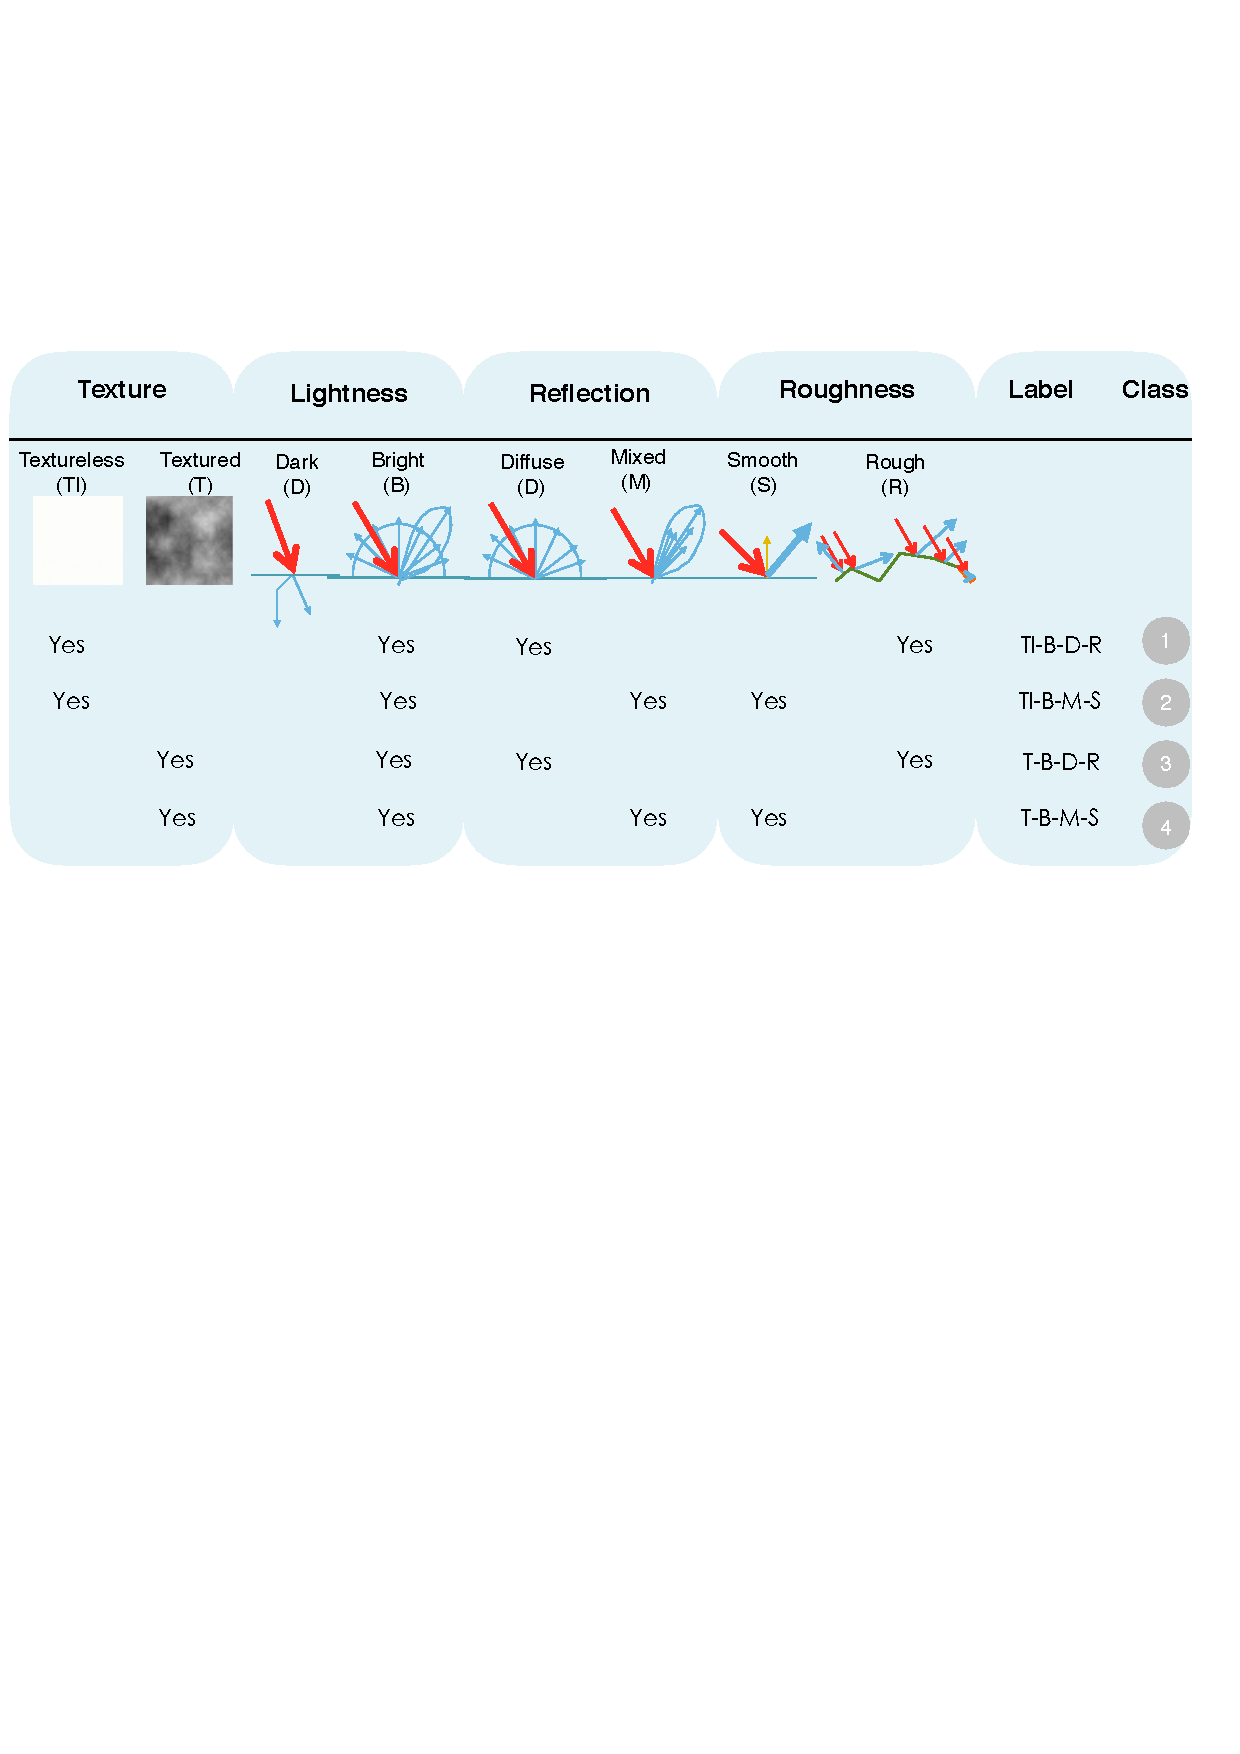
\includegraphics[width=\textwidth]{prob_space/prob_cond}
\caption{Four classes of problem conditions of interest with the proposed label.}
\label{fig:prob_cond}
\end{figure*}